\documentclass{beamer}



%%% Choose a language %%%

\newif\ifEN
\ENtrue   % uncomment this for english
%\ENfalse   % uncomment this for czech

%%% Configuration of the title page %%%

\newif\ifMFF
%\MFFtrue % comment this out for the version with a big UK university logo
\def\UKName{Charles University in Prague} %this is used in UK-logo-version
\def\UKFaculty{Faculty of Science}
\def\ThesisTypeName{\ifEN BACHELOR THESIS \else BAKALÁŘSKÁ PRÁCE \fi}
%\def\ThesisTypeName{\ifEN MASTER THESIS \else DIPLOMOVÁ PRÁCE \fi}
%\def\ThesisTypeName{\ifEN RIGOROUS THESIS \else RIGORÓZNÍ PRÁCE \fi}
%\def\ThesisTypeName{\ifEN DOCTORAL THESIS \else DISERTAČNÍ PRÁCE \fi}
\def\SupervisedThesisName{\ifEN bachelor \else bakalářské \fi}
%\def\SupervisedThesisName{\ifEN master \else diplomové \fi}
%\def\SupervisedThesisName{\ifEN rigorous \else rigorózní \fi}
%\def\SupervisedThesisName{\ifEN doctoral \else disertační \fi}


%%% Fill in your details %%%

% (Note: \xxx is a "ToDo label" which makes the unfilled visible. Remove it.)
\def\ThesisTitle{The influence of non-domain regions' composition on the activity of multi-domain protein kinases}
\def\ThesisAuthor{Jan Hamalčík}
\def\YearSubmitted{2020}

% department assigned to the thesis
\def\Department{Department of Cell Biology}
% Is it a department (katedra), or an institute (ústav)?
\def\DeptType{Department}

\def\Supervisor{doc. RNDr. Jiří Vondrášek, CSc.}
\def\SupervisorsDepartment{Institute of Organic Chemistry and Biochemistry of the CAS}

% Study programme and specialization
\def\StudyProgramme{Bioinformatics}
\def\StudyBranch{Bioinformatics}

\def\Dedication{%
Dedication. \xxx{It is nice to say thanks to supervisors, friends, family, book authors and food providers.}
}

\def\Abstract{%
\xxx{Abstracts are an abstract form of art. Use the most precise, shortest sentences that state what problem the thesis addresses, how it is approached, pinpoint the exact result achieved, and describe the applications and significance of the results. Highlight anything novel that was discovered or improved by the thesis. Maximum length is 200 words, but try to fit into 120. Abstracts are often used for deciding if a reviewer will be suitable for the thesis; a well-written abstract thus increases the probability of getting a reviewer who will like the thesis.}
% ABSTRACT IS NOT A COPY OF YOUR THESIS ASSIGNMENT!
}

% 3 to 5 keywords (recommended), each enclosed in curly braces.
% Keywords are useful for indexing and searching for the theses by topic.
\def\Keywords{%
{protein domains}, {multi-domain proteins}, {protein function}, {non-domain regions}, {protein kinases}
}

% If your abstracts are long and do not fit in the infopage, you can make the
% fonts a bit smaller by this setting. (Also, you should try to compress your abstract more.)
% Alternatively, consider increasing the size of the page by uncommenting the
% geometry modification in thesis.tex.
\def\InfoPageFont{}
%\def\InfoPageFont{\small}  %uncomment to decrease font size

\ifEN\relax\else
% If you are writing a czech thesis, you additionally need to fill in the
% english translation of the metadata here!
\def\ThesisTitleEN{\xxx{Thesis title in English}}
\def\DepartmentEN{\xxx{Name of the department in English}}
\def\DeptTypeEN{\xxx{Department}}
\def\SupervisorsDepartmentEN{\xxx{Superdepartment}}
\def\StudyProgrammeEN{\xxx{study programme}}
\def\StudyBranchEN{\xxx{study branch}}
\def\AbstractEN{%
\xxx{Abstract.}
}
\def\KeywordsEN{%
\xxx{{key} {words}}
}
\fi


\usepackage[utf8]{inputenc}

\usetheme{Berlin}

\title{\ThesisTitle}
\subtitle{\ThesisTypeName}
\author[\ThesisAuthor]{\ThesisAuthor \\ \small Supervisor: \Supervisor}
\institute[\UKFaculty]{\UKName \\ \UKFaculty}
\date{September 15\textsuperscript{th}, 2020}

\begin{document}

  \frame{\titlepage}

  \begin{frame}
    \frametitle{Overview}

    \begin{itemize}
      \item Hypothesis: General linker composition traits influence the function and
      specificity of the adjoint domains.
      \item Key consequence: Prediction of protein domain function based on the analysis
      of the non-domain regions.
      \item Method: On human two-domain proteins with one PK domain do:
        \begin{enumerate}
          \item acquire physicochemical attributes of the linkers and average them over
          their sequences,
          \item cluster the proteins by the averaged physicochemical attributes,
          \item embed GO terms and EC numbers into the clustering.
        \end{enumerate}
      \item Result: No colocalization of like GO or EC terms associated with proteins with
      different architectures was observed.
    \end{itemize}

  \end{frame}

  \begin{frame}
    \frametitle{Protein kinase domain}

    \begin{columns}

      \begin{column}{0.5\textwidth}
        \begin{itemize}
          \item Large and diverse family, involved in signal transduction.
          \item Phosphate group transfer from a phosphate donor onto a substrate.
          \item Bilobal structure with following conserved regions:
          \begin{itemize}
            \item Gly-X-Gly-X-X-Gly motif
            \item Invariant lysine
            \item DFG motif
            \item APE motif
          \end{itemize}
        \end{itemize}
      \end{column}

      \begin{column}{0.5\textwidth}
        \begin{center}
          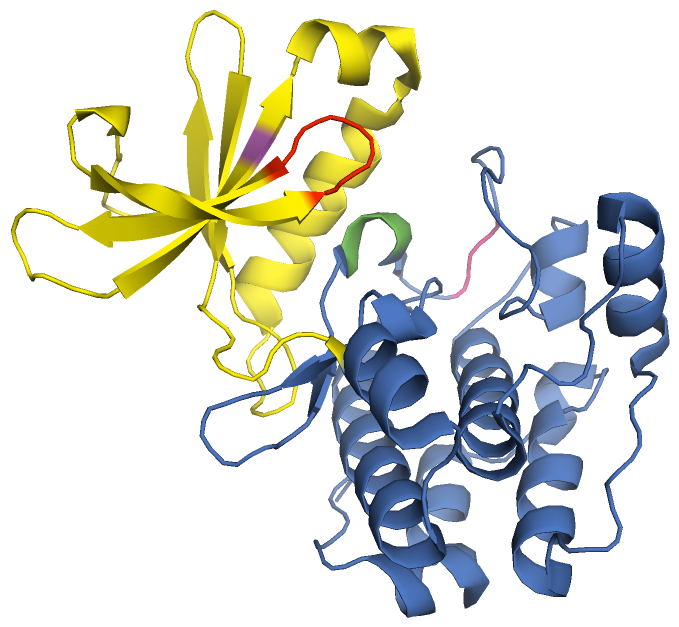
\includegraphics[width=\textwidth]{img/aurora.png}
        \end{center}
      \end{column}

    \end{columns}

  \end{frame}

  \begin{frame}
    \frametitle{Dataset}

    \begin{itemize}
      \item 117 human two-domain proteins with one PK domain
      \item 32 different architectures
      \item Averaged physicochemical attributes of their inter-domain regions:
      \begin{itemize}
        \item logarithm of the linker sequence length
        \item isoelectric point
        \item percentage of charged amino acids
        \item GRAVY index
      \end{itemize}
    \end{itemize}

    \vspace{5mm}

    2D representation of the feature space performed by UMAP.

  \end{frame}

  \begin{frame}[plain]
    \begin{center}
      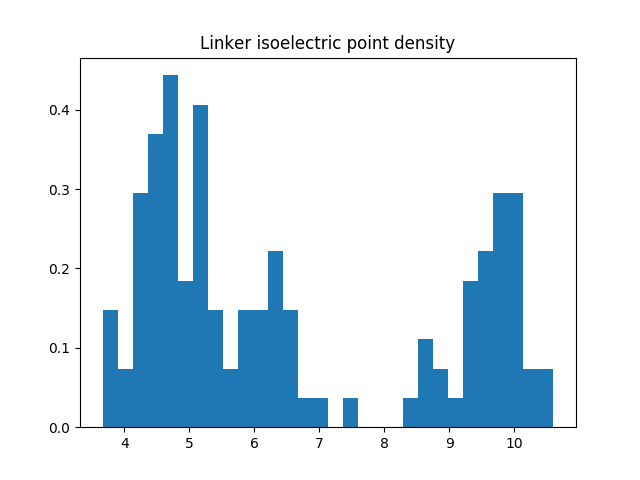
\includegraphics[width=\textwidth]{img/iso_density.png}
    \end{center}
  \end{frame}

  \begin{frame}[plain]
    \begin{center}
      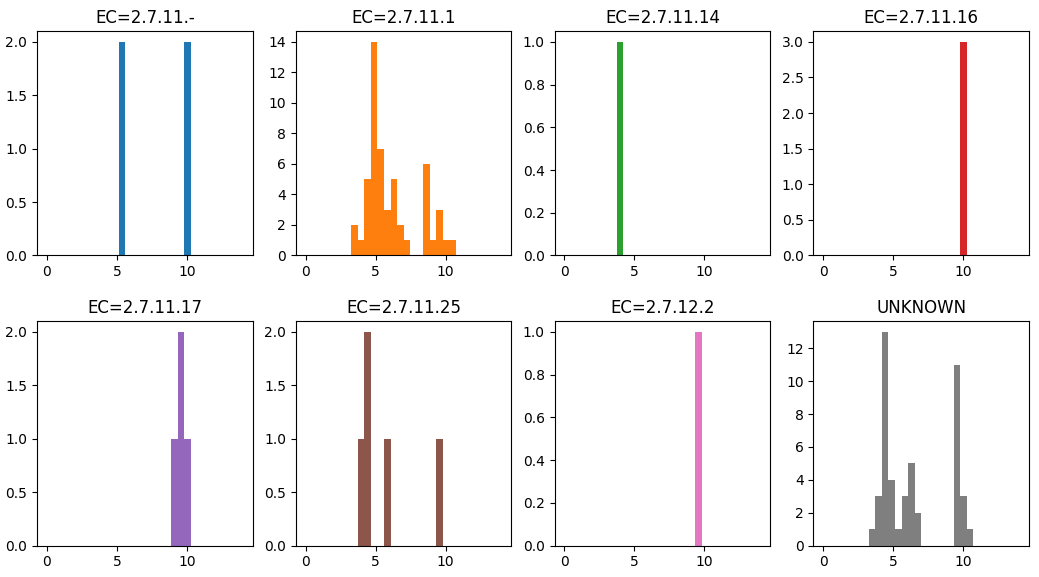
\includegraphics[width=\textwidth]{img/iso_density_ec.png}
    \end{center}
  \end{frame}

  \begin{frame}[plain]
    \begin{center}
      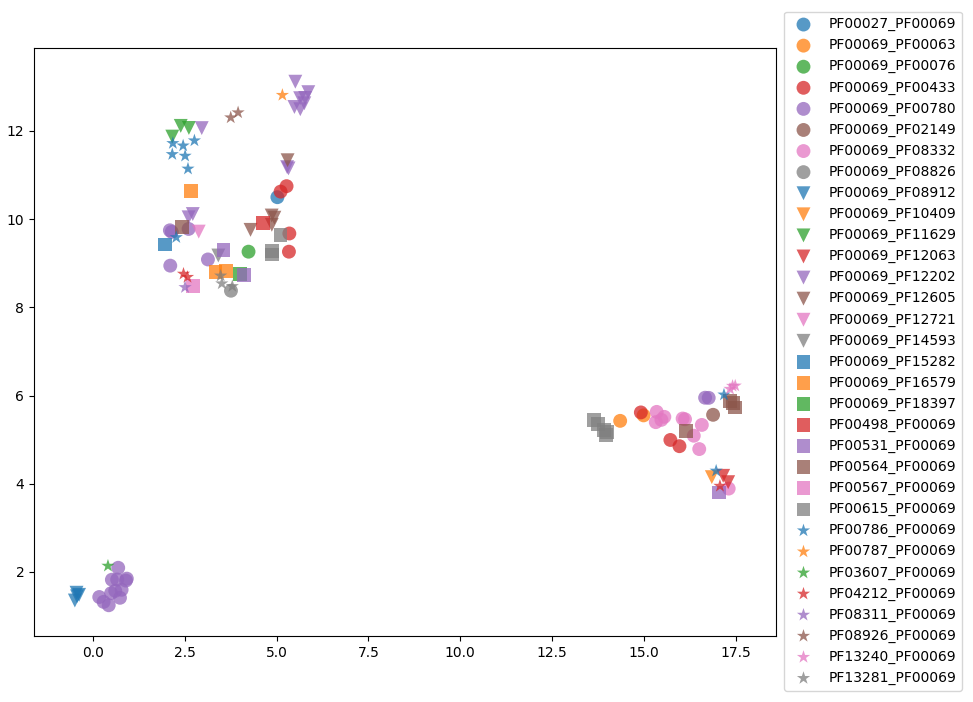
\includegraphics[width=\textwidth]{img/linker_umap_arch.png}
    \end{center}
  \end{frame}

  \begin{frame}[plain]
    \begin{center}
      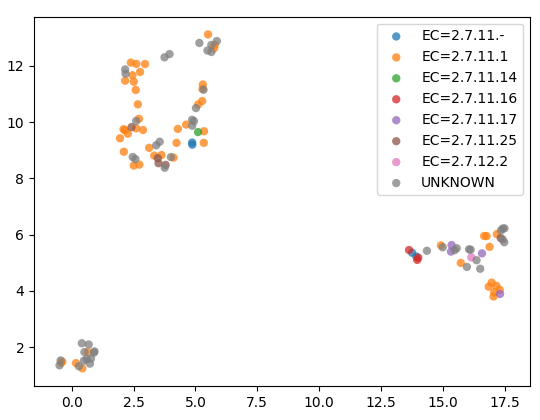
\includegraphics[width=\textwidth]{img/linker_umap_ec.png}
    \end{center}
  \end{frame}

  \begin{frame}
    \frametitle{Conclusion}

    \begin{itemize}
      \item No general influence of the linkers' composition on the overall protein
      function observed.
      \item Problems:
      \begin{itemize}
        \item 3.65625 proteins per architecture on average
        \item GO and EC are too general and too precise, respectively
        \item Observed linker types are determined by UMAP parametrization
      \end{itemize}
    \end{itemize}
  \end{frame}

\end{document}
